\hypertarget{web-checkers-design-documentation}{%
\section{Web Checkers Design
Documentation}\label{web-checkers-design-documentation}}

\hypertarget{team-information}{%
\subsection{Team Information}\label{team-information}}

\usepackage{float}

\begin{itemize}
\tightlist
\item
  Team name: thePurpleNarwhals
\item
  Team members

  \begin{itemize}
  \tightlist
  \item
    Michael Taylor
  \item
    Greg Villafane
  \item
    Huan Huynh
  \item
    Andrew Chacon
  \end{itemize}
\end{itemize}

\hypertarget{executive-summary}{%
\subsection{Executive Summary}\label{executive-summary}}

The application must allow players to play checkers with other players
who are currently signed in. The game user interface (UI) will support a
game experience using drag-and-drop browser capabilities for making
moves. Beyond this minimal set of features, we have grand vision for how
we could further enhance the player experience with some additional
features beyond the basic checkers game.

\hypertarget{purpose}{%
\subsubsection{Purpose}\label{purpose}}

Create a web-based Checkers game using Maven and Freemarker,
implementing the game through frontend and backend development. Each
player should be able to successfully play a game of checkers.

\hypertarget{glossary-and-acronyms}{%
\subsubsection{Glossary and Acronyms}\label{glossary-and-acronyms}}

\begin{longtable}[]{@{}ll@{}}
\toprule
Term & Definition \\
\midrule
\endhead
VO & Value Object \\
\bottomrule
\end{longtable}

\hypertarget{requirements}{%
\subsection{Requirements}\label{requirements}}

This section describes the features of the application.

\hypertarget{definition-of-mvp}{%
\subsubsection{Definition of MVP}\label{definition-of-mvp}}

A user should be able to sign in to start playing checkers. A user once
signed in can start a game with another player. Each player should be
able to play a standard game of checkers and have the option to resign
during the game.

\hypertarget{mvp-features}{%
\subsubsection{MVP Features}\label{mvp-features}}

\begin{itemize}
\tightlist
\item
  As a user I want to be able to sign in with the desired username of my
  choice.
\item
  As a user I want to be able to start a game and play with another.
\item
  As a user I want to be able to move a piece when I drag a piece to a
  valid square.
\item
  As a user I want to be able to capture a piece when I drag a piece
  over an opponent's piece.
\item
  As a user I want to be able to forfeit the game when I feel helpless
  to end the game.
\end{itemize}

\hypertarget{roadmap-of-enhancements}{%
\subsubsection{Roadmap of Enhancements}\label{roadmap-of-enhancements}}

\begin{itemize}
\tightlist
\item
  Provide a button to give a hint to the Player.
\item
  The hint will return a list of possible moves the PLayer can make.
\item
  The Player can start multiple games at the same time and switch
  between the games.
\end{itemize}

\hypertarget{application-domain}{%
\subsection{Application Domain}\label{application-domain}}

This section describes the application domain.

\begin{figure}[H]
\centering
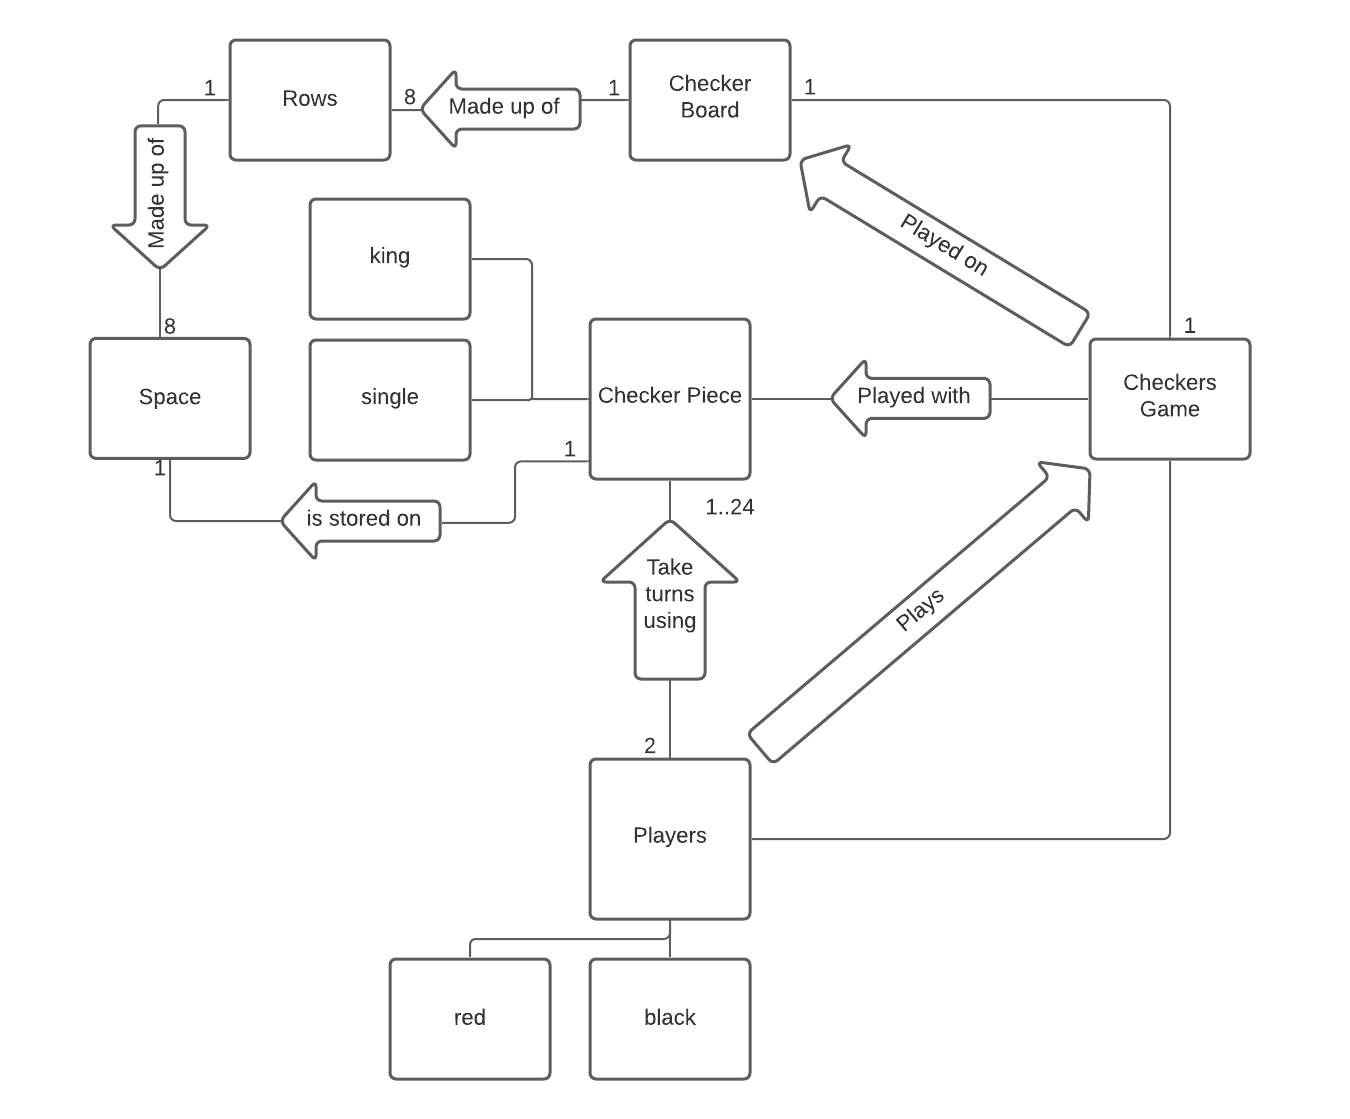
\includegraphics{domain-model.png}
\caption{The WebCheckers Domain Model}
\end{figure}

A list of Players will be in a menu after signing in. A Player will play
a Checkers game, making the move using the pieces. The Game has a Board
for the game to be played on. The Board is made up of Rows and Spaces,
which the pieces will be stored on. The Player can then make a Move to
progress the game. A Player can play multiple games at the same time and
also get a hint during the game.

\hypertarget{architecture-and-design}{%
\subsection{Architecture and Design}\label{architecture-and-design}}

This section describes the application architecture.

\hypertarget{summary}{%
\subsubsection{Summary}\label{summary}}

The following Tiers/Layers model shows a high-level view of the webapp's
architecture.

\begin{figure}[H]
\centering
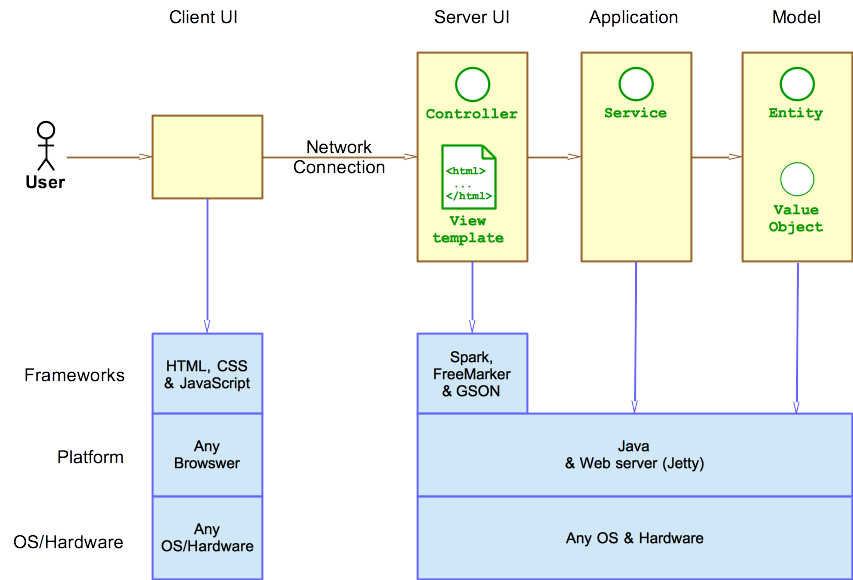
\includegraphics{architecture-tiers-and-layers.png}
\caption{The Tiers \& Layers of the Architecture}
\end{figure}

As a web application, the user interacts with the system using a
browser. The client-side of the UI is composed of HTML pages with some
minimal CSS for styling the page. There is also some JavaScript that has
been provided to the team by the architect.

The server-side tiers include the UI Tier that is composed of UI
Controllers and Views. Controllers are built using the Spark framework
and View are built using the FreeMarker framework. The Application and
Model tiers are built using plain-old Java objects (POJOs).

Details of the components within these tiers are supplied below.

\hypertarget{overview-of-user-interface}{%
\subsubsection{Overview of User
Interface}\label{overview-of-user-interface}}

This section describes the web interface flow; this is how the user
views and interacts with the WebCheckers application.

\begin{figure}[H]
\centering
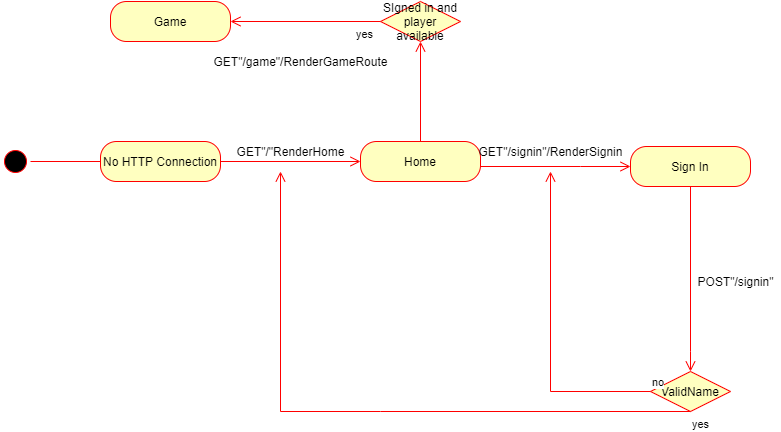
\includegraphics{web-interface.png}
\caption{The WebCheckers Web Interface Statechart}
\end{figure}

The user will go to the home page when first coming to the application.
The user will then be able to get to the /signin page. If the name
entered is valid, then they will be taken to the /home page. If the name
entered is invalid, then they will stay at the /signin page. When the
user is signed in and at the home page, the user will then be able to
get to the /game page to play a game. \texttt{GET\ /GameRoute} is called
to begin the game. Drag and drop mechanics are used to move the checkers
from square to square. Buttons are used to submit the turn, undo the
move, resign the game, and receive a hint. The page will refresh
periodically to update the board once the opponent submits their turn or
resigns the game.

\hypertarget{ui-tier}{%
\subsubsection{UI Tier}\label{ui-tier}}

Provide summary, add sequence diagrams/statecharts, go through what gets
called as the game progresses.

The UI is composed of the routes needed to properly navigate the website
and play the game. All routes created inherit from the \texttt{Route}
interface. The user starts at the home route, then \texttt{GET\ /signin}
is called to allow the user to log in. After a successful log-in, the
user is taken back to the homepage, where \texttt{GET\ /GameRoute} is
called when a Player clicks on another Player to begin the game.

In the Game, if it is your turn, when a move is made,
\texttt{POST\ /ValidateMove} is called which will verify the move is
legal. If the move is legal and the submit button is pressed, then
\texttt{POST\ /SubmitTurn} is called, which will update the board and
allow the opponent to move. This process repeats until the game is over.
Figure 4 shows the sequence diagram of \texttt{PostValidateMoveRoute}.

\begin{figure}[H]
\centering
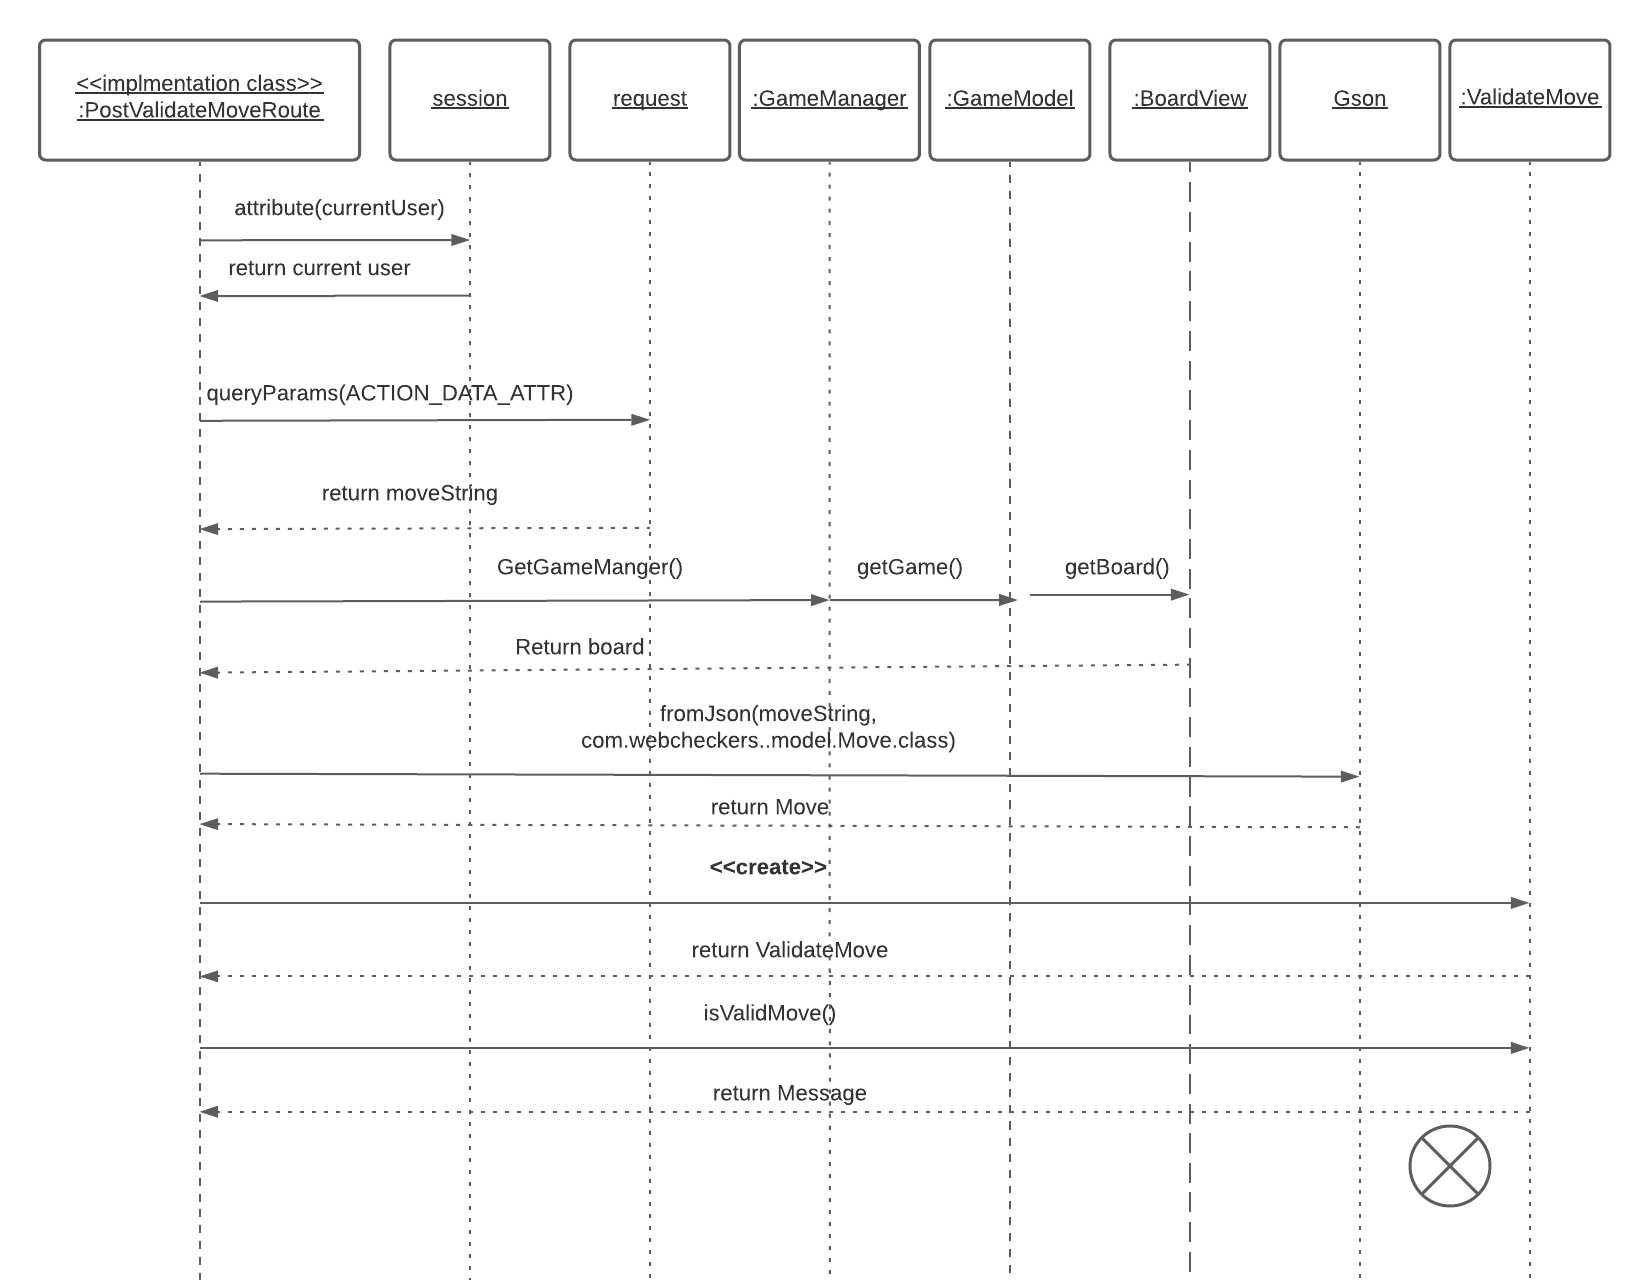
\includegraphics{validateMoveSD.png}
\caption{Sequence Diagram for PostValidateMoveRoute}
\end{figure}

If a move is made and the Player wants to undo the move, then
\texttt{PostBackupMoveRoute} is called, which puts the board back in its
previous state. If the Player wants a hint, then
\texttt{PostMakeHintRoute} is called, which will generate the hint and
return it to the board. Figure 5 shows the connection of these routes.

\begin{figure}[H]
\centering
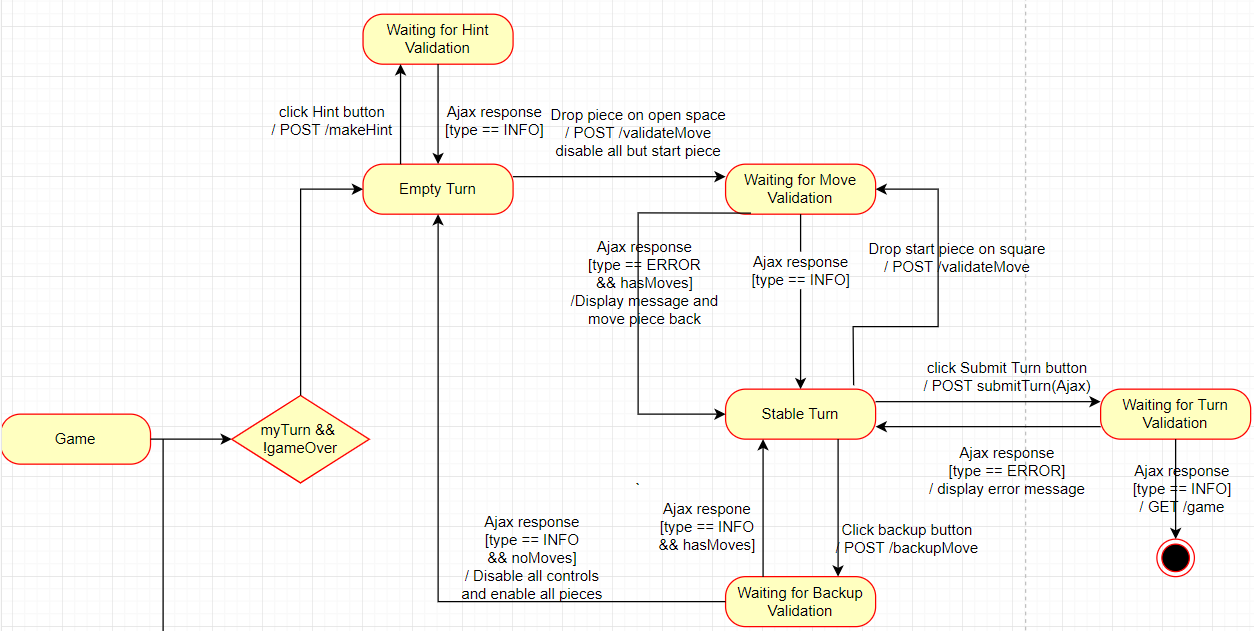
\includegraphics{myTurn-statechart.png}
\caption{Statechart of making a turn}
\end{figure}

If it is not your turn, then the page will continuously refresh until
the turn updates. This is done by calling \texttt{PostCheckTurnRoute}
every 5 seconds to refresh the page. If it is the end of the game, then
\texttt{PostResignGameRoute} is called to end the game, which updates
the Game page and hides all buttons except the button to exit the game.

\hypertarget{application-tier}{%
\subsubsection{Application Tier}\label{application-tier}}

When a user goes to sign in, their name is put in the
\texttt{PlayerLobby} to be stored. If the name entered is already in the
lobby, then the name is invalid and the user will have to use a
different name to sign in. When a game is started, the
\texttt{GameManager} will put the players in a game and create the
board.

\hypertarget{model-tier}{%
\subsubsection{Model Tier}\label{model-tier}}

When a user successfully signs in, they now become a \texttt{Player} in
the lobby. When the players start a game, the \texttt{Boardview}
represents the board, which consists of \texttt{Row}s and
\texttt{Space}s, which the \texttt{Piece}s are then placed on. A
\texttt{GameModel} is also used to represent one game. When a move is
made on the board, a \texttt{Move} is created, which contains the start
and end \texttt{Position} of the piece moved. The \texttt{ValidateMove}
class is then used to verify whether the move was valid. If the user
requests it, a hint can be made using \texttt{MakeHint}.

\begin{figure}
\centering
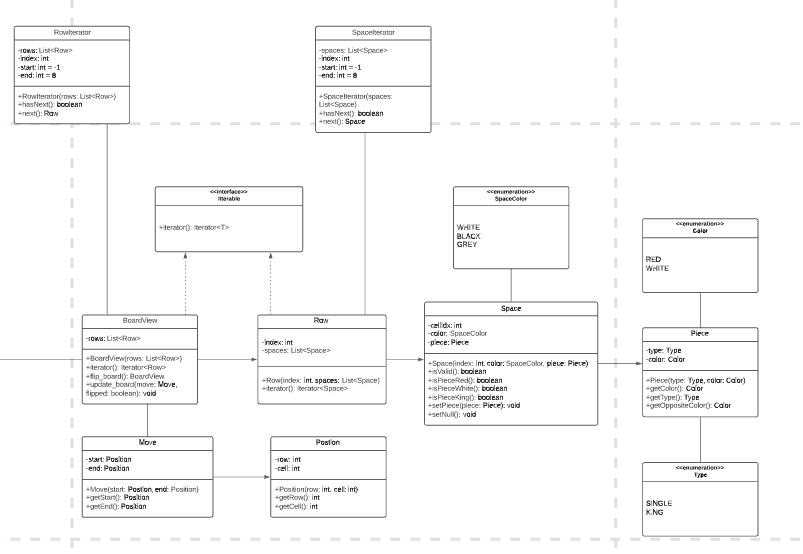
\includegraphics{boardUML.png}
\caption{UML Diagram for the checkers board}
\end{figure}

\hypertarget{design-improvements}{%
\subsubsection{Design Improvements}\label{design-improvements}}

While Object-Oriented principles are followed, the use and consistency
of them are not apparent throughout the architecture. The Law of
Demeter, in particular, is a principle that could be improved throughout
the design. In addition, there are some classes that have been replaced
with new classes, but have not been removed from the architecture. This
causes issues with coupling and can be fixed by replacing the obsolete
classes with their successor in the design, as well as implementing more
abstraction so the issue can be avoided in the future. In addition,
refactoring can be done to separate concerns within the main tiers.
Classes within the tiers should be put into packages to separate classes
that focus on different aspects of the program.

In addition, the code metrics yield some areas of improvement across
multiple categories. The lines of code metric show that each class has
at most 139 lines of code, with one exception. \texttt{ValidateMove} has
238 lines of code, which is high compared to the rest of the project.
This can be fixed by breaking the class in to smaller classes. The
complexity metric show that \texttt{ValidateMove} and
\texttt{GetGameRoute} are more complex than the rest of the classes.
This is due to the complexity of the methods involved in the classes.
This can be fixed by breaking down the methods within the class or
breaking up the responsibility of the class in to smaller classes. The
Chidamber-Kemerer metric show that \texttt{ValidateMove} has a high
method complexity relative to the rest of the classes. In addition, the
classes have good cohesion with each other. The Javadoc metric show that
comments are sparse throughout the project and could be improved upon.
The Martin packaging metrics show that the UI tier calls from classes
that are outside the package and the Model tier has methods that are
called from outside the package. This shows that data from the Model
tier is exchanged heavily with the UI tier. In addition, the application
tier has coupling with the other tiers. The number of calls can be
reduced by creating controller classes in each package that will handle
any data that must be communicated between packages. This will funnel
the transfer of data and reduce coupling between the packages.

\hypertarget{testing}{%
\subsection{Testing}\label{testing}}

Unit testing was performed on some of the UI tier and the Application
tier. Acceptance testing was also made for each story.

\hypertarget{acceptance-testing}{%
\subsubsection{Acceptance Testing}\label{acceptance-testing}}

Eight user stories have passed all of their acceptance testing and one
story has an acceptance criteria that failed. This criteria failed
during the implementation of multiple games. The user will not
automatically be pulled in to a game if an opponent starts a game.
Instead, a button showing the players are in a game will appear and the
user must click the button to enter the game. This can be fixed,
however. There were no issues that occurred with testing, except for
what was mentioned, and there are no concerns with the final product in
terms of the acceptance criteria.

\hypertarget{unit-testing-and-code-coverage}{%
\subsubsection{Unit Testing and Code
Coverage}\label{unit-testing-and-code-coverage}}

In order to ensure the functionality of the features, unit testing was
neglected throughout the project. Minimal testing was performed, with
the Application tier tested, the Model tier partially tested, and the UI
tier minimally tested. The Application tier has 84\% coverage, the Model
tier has 44\% coverage, and the UI tier has only 6\% coverage. This is a
clear area for improvement in the project.
